% !TEX program = lualatex
\documentclass[12pt,a4paper]{article}
\usepackage{fontspec}
\setmonofont{Latin Modern Mono}
\usepackage{xcolor}
\usepackage{listings}
\usepackage{geometry}
\usepackage{fancyhdr}
\usepackage{hyperref}
\usepackage{graphicx}
\usepackage{multicol}
\geometry{margin=1in}

% -------------------------------
% SOLUTION TOGGLE
% -------------------------------
\newif\ifshowsolutions
\showsolutionstrue        
% \showsolutionsfalse    

% -------------------------------
% Header and Footer Configuration
% -------------------------------
\pagestyle{fancy}
\fancyhf{}
\lhead{Lab Mid}
\rhead{CSE 4308: DBMS Lab}
\cfoot{\thepage}
\setlength{\headwidth}{\textwidth}

% -------------------------------
% Code Listing Style
% -------------------------------
\definecolor{codegreen}{rgb}{0,0.6,0}
\definecolor{codegray}{rgb}{0.5,0.5,0.5}
\definecolor{codepurple}{rgb}{0.58,0,0.82}
\definecolor{backcolour}{rgb}{0.95,0.95,0.92}

\lstdefinestyle{mystyle}{
    backgroundcolor=\color{backcolour},
    commentstyle=\color{codegreen},
    keywordstyle=\color{magenta},
    numberstyle=\tiny\color{codegray},
    stringstyle=\color{codepurple},
    basicstyle=\ttfamily\footnotesize,
    breaklines=true,
    captionpos=b,
    keepspaces=true,
    numbers = none,
    numbersep=5pt,
    tabsize=2,
    frame=single,
    columns=fullflexible,
    showspaces=false,
    showstringspaces=false,
    showtabs=false
}

\lstset{style=mystyle}

% Images: found next to this file (local compile_labs.sh) or via the
% lab folder when compiled from the project root (Overleaf).
\graphicspath{{lab_08_mid/}}

\begin{document}

% --------------------------------------------------------------
% TITLE PAGE
% --------------------------------------------------------------
\begin{titlepage}
    \centering
    \vspace*{2\baselineskip}

    \rule{14cm}{2pt}\vspace*{-0.8\baselineskip}\vspace*{1.5pt}
    \rule{14cm}{0.5pt}\vspace{2\baselineskip}

    {\Huge\bfseries\scshape Lab Mid\par}

    \rule{14cm}{0.5pt}\vspace*{-0.7\baselineskip}\vspace{2.5pt}
    \rule{14cm}{2pt}

    \vspace{2\baselineskip}

    {\Large\bfseries CSE 4308\par}
    \vspace{1\baselineskip}
    {\large DATABASE MANAGEMENT SYSTEMS LAB\par}

    \vfill
    {\normalsize Prepared by:\\ Samnun Azfar, Jr. Lecturer, CSE\\ Samia Nawsheen, Jr. Lecturer, CSE\par}
    {\normalsize Academic Year: AY25-26\par}
\end{titlepage}

\newpage

% ==============================================================
\section*{DBMS Lab Mid}

\begin{figure}[h]
    \centering
    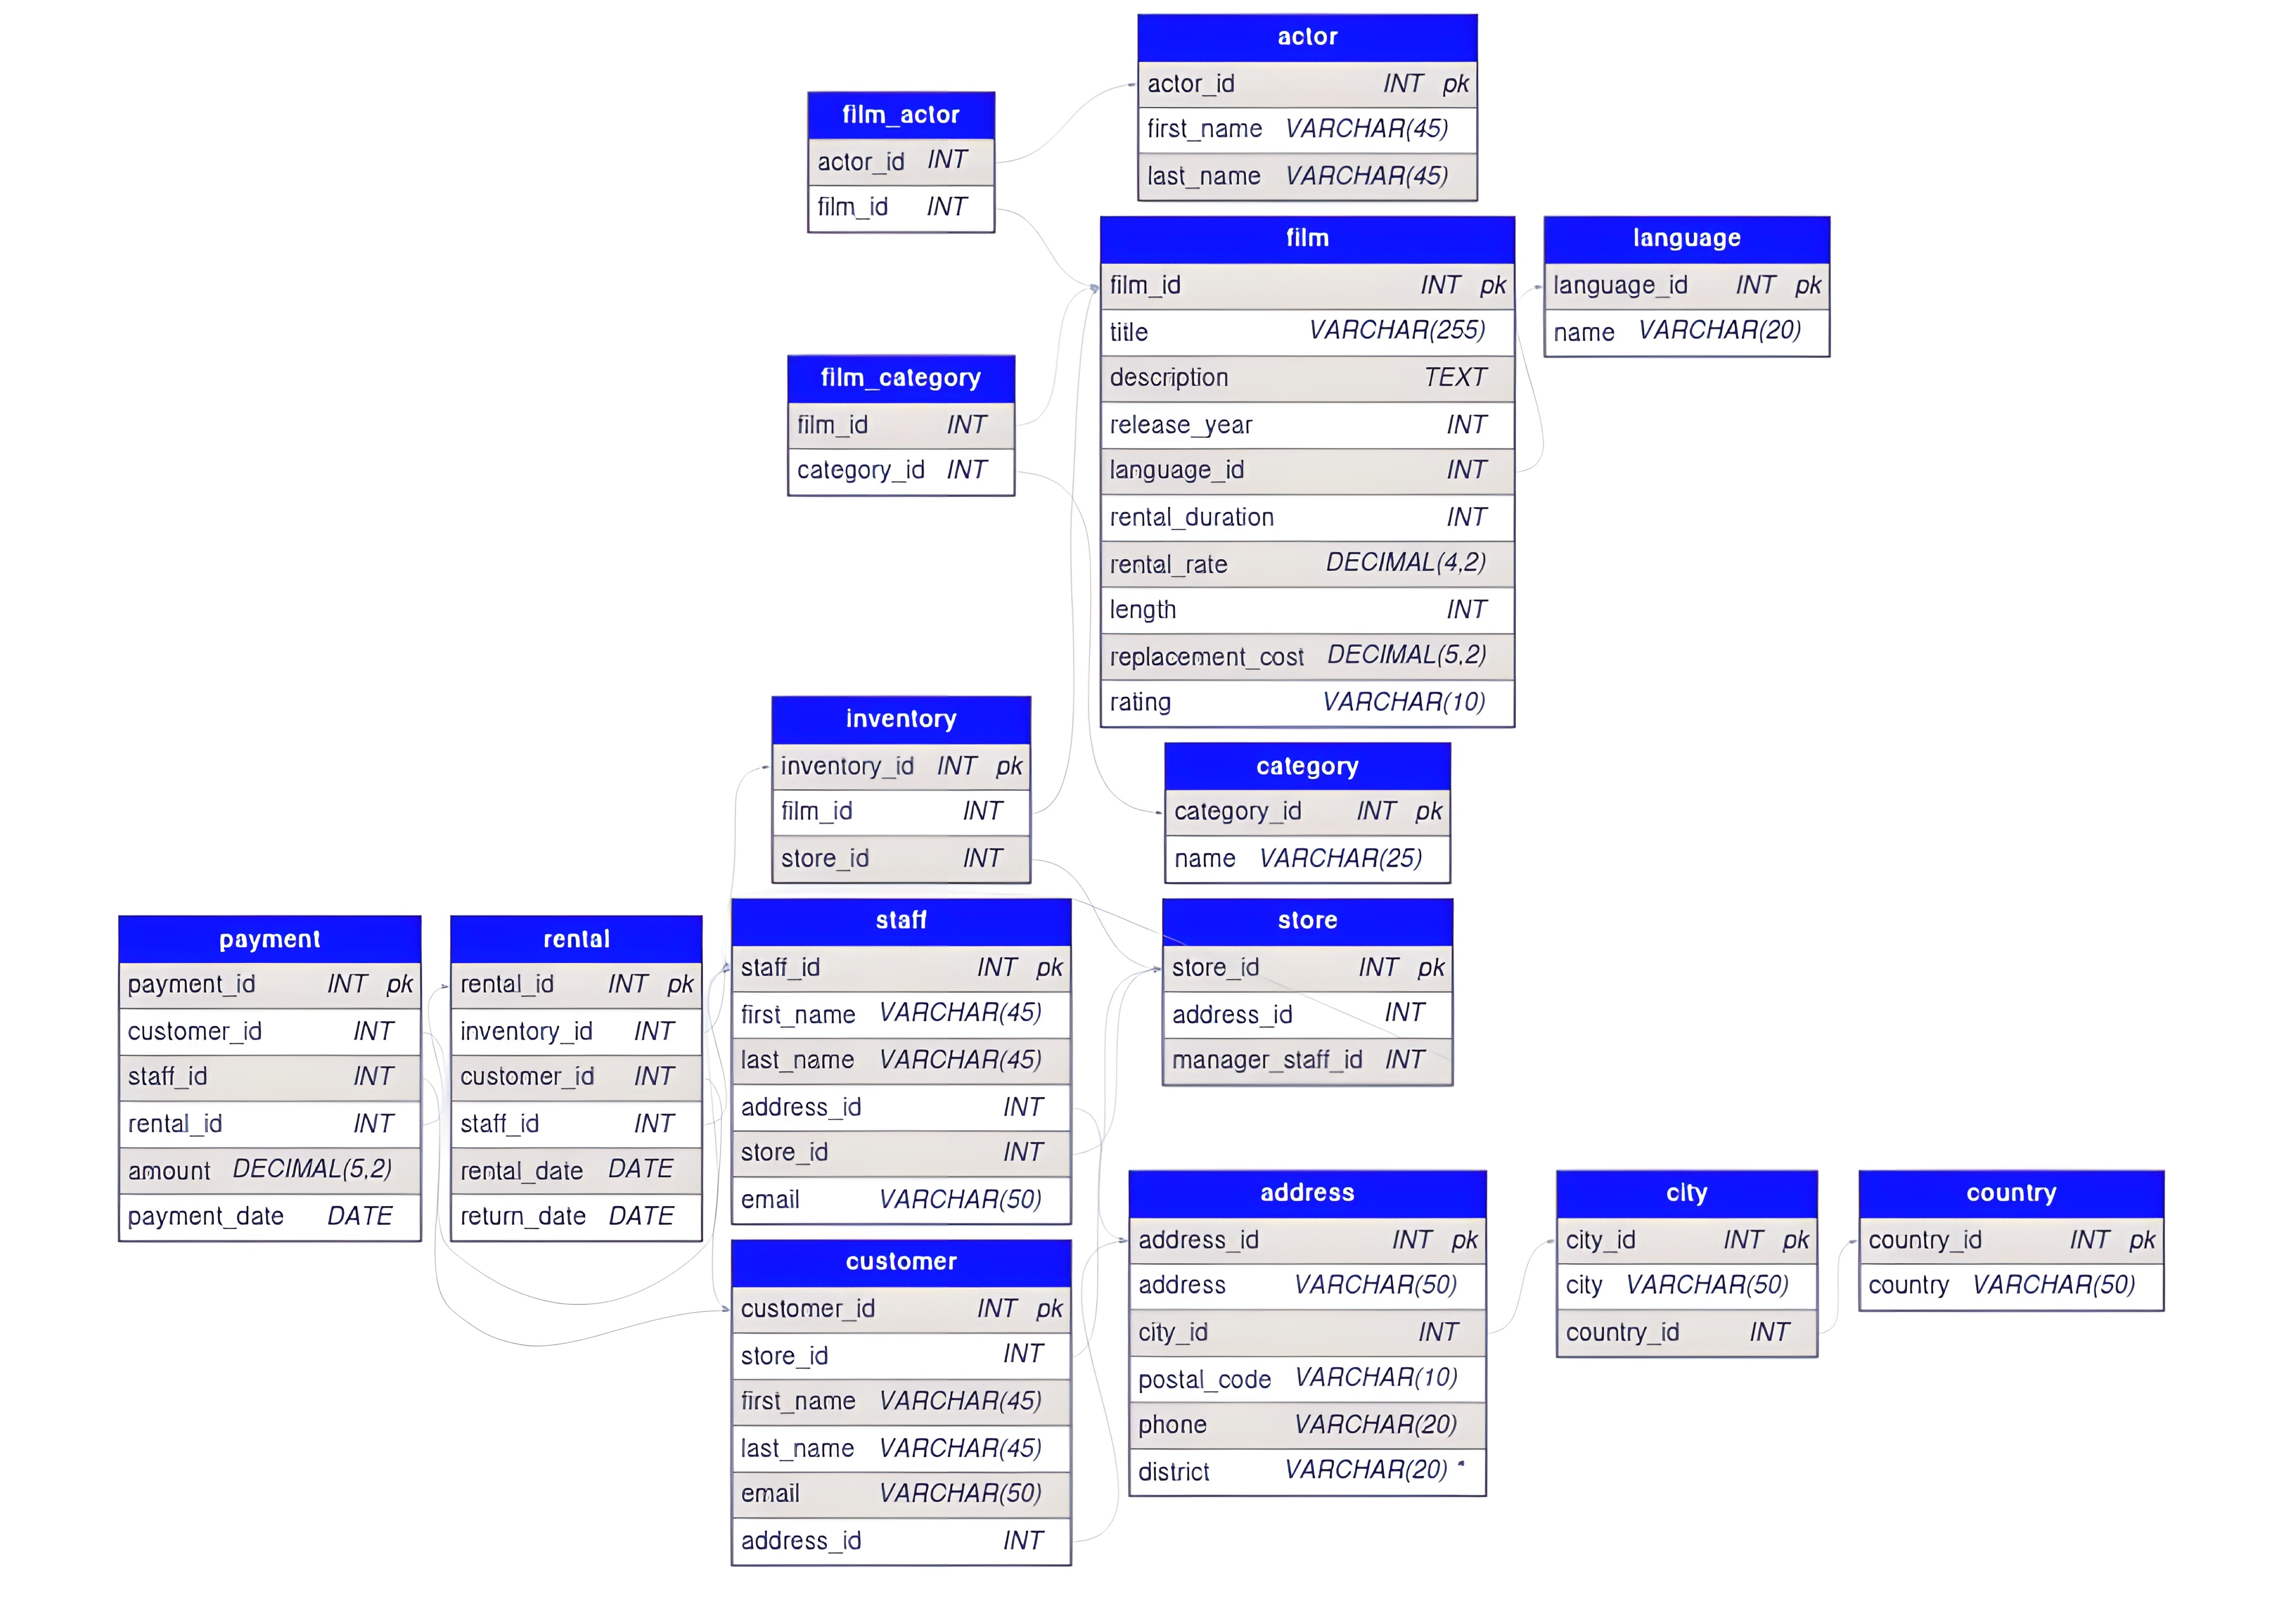
\includegraphics[width=\linewidth]{lab_08_dvdrental_1.png}
\end{figure}

\begin{enumerate}

\item Display the film title and release year for all films released after 2005.

\ifshowsolutions
\begin{lstlisting}[language=SQL]
SELECT title, release_year
FROM film
WHERE release_year > 2005;
\end{lstlisting}
\fi

\item For each district, show the number of customers living there. Only include districts with more than 5 customers.

\ifshowsolutions
\begin{lstlisting}[language=SQL]
SELECT a.district, COUNT(c.customer_id) AS customer_count
FROM customer c
JOIN address a ON c.address_id = a.address_id
GROUP BY a.district
HAVING COUNT(c.customer_id) > 5;
\end{lstlisting}
\fi

\item List all stores along with the total number of inventory items they have.

\ifshowsolutions
\begin{lstlisting}[language=SQL]
SELECT s.store_id, COUNT(i.inventory_id) AS total_inventory
FROM store s
LEFT JOIN inventory i ON s.store_id = i.store_id
GROUP BY s.store_id;
\end{lstlisting}
\fi

\item For each film rating (G, PG, PG-13, R), calculate the average rental rate.

\ifshowsolutions
\begin{lstlisting}[language=SQL]
SELECT rating, AVG(rental_rate) AS avg_rental_rate
FROM film
WHERE rating IN ('G', 'PG', 'PG-13', 'R')
GROUP BY rating
ORDER BY rating;
\end{lstlisting}
\fi

\item List rentals where the rental month and return month are the same.

\ifshowsolutions
\begin{lstlisting}[language=SQL]
SELECT rental_id, rental_date, return_date
FROM rental
WHERE EXTRACT(MONTH FROM rental_date) =
      EXTRACT(MONTH FROM return_date);
\end{lstlisting}
\fi

\item Find all customers whose first names start with \texttt{A} and whose emails contain \texttt{.org}.

\ifshowsolutions
\begin{lstlisting}[language=SQL]
SELECT first_name, last_name, email
FROM customer
WHERE LOWER(first_name) LIKE 'a%'
  AND LOWER(email) LIKE '%.org%';
\end{lstlisting}
\fi

\item Display the customer ID and email for customers whose email length is greater than 20 characters.

\ifshowsolutions
\begin{lstlisting}[language=SQL]
SELECT customer_id, email
FROM customer
WHERE LENGTH(email) > 20;
\end{lstlisting}
\fi

\item Display each film title along with the total number of copies available in inventory.

\ifshowsolutions
\begin{lstlisting}[language=SQL]
SELECT f.title, COUNT(i.inventory_id) AS total_copies
FROM film f
JOIN inventory i ON f.film_id = i.film_id
GROUP BY f.film_id, f.title
ORDER BY total_copies DESC;
\end{lstlisting}
\fi

\item Find the actors who acted in both \texttt{Comedy} and \texttt{Action} films.

\ifshowsolutions
\begin{lstlisting}[language=SQL]
SELECT a.actor_id, a.first_name, a.last_name
FROM actor a
WHERE a.actor_id IN (
    SELECT actor_id
    FROM film_actor fa
    JOIN film_category fc ON fa.film_id = fc.film_id
    JOIN category c ON fc.category_id = c.category_id
    WHERE c.name = 'Comedy'
)
AND a.actor_id IN (
    SELECT actor_id
    FROM film_actor fa
    JOIN film_category fc ON fa.film_id = fc.film_id
    JOIN category c ON fc.category_id = c.category_id
    WHERE c.name = 'Action'
);
\end{lstlisting}
\fi

\item For each store, find the customer(s) who made the highest number of rentals in that store. 
\ifshowsolutions
\begin{lstlisting}[language=SQL]
SELECT i.store_id, c.first_name, c.last_name, COUNT(*) AS rental_count
FROM inventory i
JOIN rental r ON i.inventory_id = r.inventory_id
JOIN customer c ON r.customer_id = c.customer_id
GROUP BY i.store_id, c.customer_id, c.first_name, c.last_name
HAVING COUNT(*) = (
    SELECT MAX(cnt)
    FROM (
        SELECT COUNT(*) AS cnt
        FROM inventory i2
        JOIN rental r2 ON i2.inventory_id = r2.inventory_id
        WHERE i2.store_id = i.store_id
        GROUP BY r2.customer_id
    ) x
);
\end{lstlisting}
\fi

\end{enumerate}

\end{document}
